\chapter{基于Hadoop的MapReduce实现的性能分析}
\label{chap:4}

\section{Hadoop调度对性能的影响}
Hadoop程序运行时,会有进程监控节点资源,并将系统中的空闲资源按一定的策略分配给作业,这个进程的核心就是调度器。Hadoop默认的调度器是JobQueueTaskScheduler,使用规则为FIFO (First In First Out,即先入先出)原则,即按照作业的优先级高低,再按照到达时间的先后选择被执行的作业。

其具体工作流程如下图\ref{fig:调度器}:
\begin{figure}[h]
 \centering
 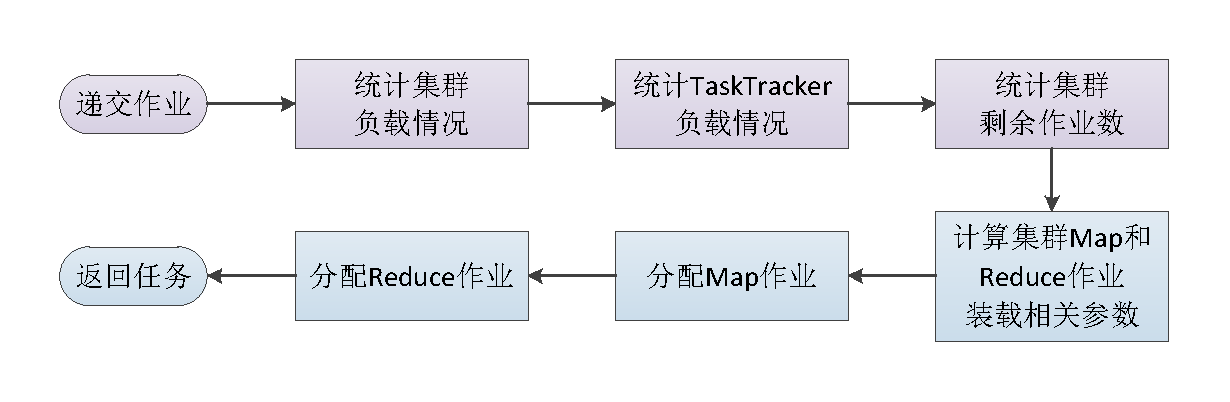
\includegraphics[width=1\textwidth]{调度器}
 \caption{调度器}
 \label{fig:调度器}
\end{figure}

对于JobQueueTaskScheduler的任务调度原则可总结如下:

\begin{enumerate}
\item 任务先进先出;
\item 尽量使集群每一个TaskTracker达到负载均衡(这个均衡是task数量上的而不是实际的工作强度);
\item 尽量分配作业的本地任务给TaskTracker,但不是尽快分配作业的本地任务给TaskTracker,最多分配一个非本地任务给TaskTracker(一是保证任务的并发性,二是避免有些TaskTracker的本地任务被偷走),最多分配一个reduce任务;
\item 为紧急的Task预留一定的slot;
\end{enumerate}

这种调度方式简单明了,JobTracker负载较小,适用于大多数的应用场景。

它的主要缺点就是对于在集群比较繁忙的情况,低优先级的作业将很难分配到集群的计算资源,这样对于那些低优先级同时又要求一定的响应时间的短作业来说是非常不利的。

为了解决这种应用差异性带来的性能损失,Hadoop允许用户自定义调度器。Hadoop的调度器被设计为一个可插拔的模块,用户可以根据自己实际应用要求设计调度器。

但由于调度机制在单机为分布式下的执行过于简单,其调度结果不具有参考价值,故在本文中不予以进一步的讨论。

\section{Hadoop运行机制对MapReduce性能的影响}
\subsection{原生Java}
通过第三章的测试结果可以看出,原生Java程序运行时,Map在经过一次大量的读操作之后,其写操作和Reduce的读写操作均经过合并优化。Map的结果被很好的合并,并交给了Reducer进行处理。程序运行效率非常高。

由于Hadoop提供了类库,所有操作均可通过接口实现,且对Hadoop内部透明,方便数据合并及优化,降低了I/O压力,性能损失很小。

\subsection{基于Streaming的实现}
通过第三章的的测试结果可以看出,基于Streaming的实现,Python的运行时间随着文件的增大逐渐比Java长,性能变差的主要是因为Map的结果没有进行combine。从表可以看出,Streaming中的Map和Reduce结果没有经过任何Combine,直接存入本地磁盘,从而造成了大量的空间浪费,增大了I/O负担,进入Reduce进一步处理的数据没有经过合并,造成性能损失。

以处理1亿条日志为例,从表可以得出,Streaming的实现与Java相比,写入量增大约100倍,读入量增大约10万倍,内存使用量增大约3倍,Reduce函数输入量增大了约15万倍,造成了性能损失。

由此可见,MapReduce框架中的输入输出优化、缓存和合并机制是MapReduce程序运行效率的关键。

\section{节点计算能力对MapReduce性能的影响}
Hadoop中,作业在TaskTracker上执行,TaskTracker的计算能力直接影响着Hadoop的整体性能。MapReduce是分布式计算框架,节点之间的通信通过网络传输。在Map和Reduce过程中,Hadoop产生了大量的网络和磁盘I/O,尤其是在Mapper和Reducer结束时,会引起数据量极大的“网络风暴”,这在实际生产环境中会给网卡和交换机带来很大的压力,若配置不当,将会成为MapReduce的瓶颈。

同时,在Hadoop运行过程中,Reduce在shuffle阶段对下载来的Map数据,并不是立刻就写入磁盘的,而是会先缓存在内存中,然后当使用内存达到一定量的时候才刷入磁盘,这就要求节点机有足够大的内存去缓存数据,默认情况下,reduce会使用其heapsize的70\%来在内存中缓存数据。内存的大小决定了缓存数量的多少,减少不必要的I/O。

磁盘读写速度也是MapReduce中影响性能的一个重要指标,在Map阶段,Hadoop会将Map的中间结果保存在节点本地磁盘,因为中间结果是临时的,不需要写多份。本地磁盘的读写I/O速度在某些应用中也会成为MapReduce程序的瓶颈。

另外,在实际生产环境中,节点计算之间的计算能力会有略微的不同,默认的Hadoop调度器会使作业运行时出现性能短板,这种短板在异构环境中尤为明显。

\section{实例程序编写方法对MapReduce性能的影响}
通过Java和Streaming两种实现方式的比较,可以看出影响MapReduce较大的部分为Suffle部分,从MapReduce运行原理可以看出,Suffle部分的合并是根据Key值合并的,如何合理的选择Key值,降低Reducer的处理时间,对MapReduce程序的运行起着至关重要的作用。

但实际开发中,Key的分布并不一定是均匀的,极端情况下,所有数据共享一个Key,后果是reduce任务只会在集群其中一个节点上运行,不仅没有利用好集群处理能力,反倒因为大量数据集中而导致计算效率低下,降低程序整体运行效率。

作为了解决这个问题,程序员需要在编程时尽量选择分布均匀的参数作为Key,或者使用其他方法将Key打散。下文以Web日志处理中的处理UV为例,描述了一种打散Key的方法。

UV是独立访客 (unique visitor)的缩写,对于网站的用户粘度和回头率统计有着至关重要的作用。

在网站设计中,通常会给Cookie一个Key为uid,Value为用户id的一组数据。在Web日志中,该uid即可用来统计UV。

在未打散Key的情况下,uid的值会比较分散,但对于游客用户来说,uid值为空,即0,这就会造成Map的结果中,uid分布不均匀。这时,将uid的值设为用户ip的后三位,从而使游客的统计均匀的分发到不同的Key中。但仅仅这样做是不够的,每个uid都不同,会导致Map结果中Key的数量过多,不便于数据合并和传输。这时,可以使用取模函数对uid取模,将Key的数量控制在合适的范围之内。进而分发到不同的Reduce节点上。

在Reduce阶段,Reducer接收到Key/Value对时,可以对Cookie值进行判断,若uid为空,则访客数+1,反之则该uid的统计数+1。

具体实现流程如下图:

实际生产环境中,Key的打散和控制还有其他多种方法,如将字符串转换为整形数字提高处理速度、或者将一个MapReduce操作划分成两份MapReduce程序去执行。具体使用方法应该根据应用程序的要求来确定,在此不一一赘述。

\section{本章小结}
本章通过分析Hadoop运行过程和运行机制,结合第\ref{chap:3}章中的测试结果,